\documentclass[11pt,a4paper]{article}
\usepackage[margin=22mm]{geometry}
\usepackage{amsmath,booktabs,graphicx,hyperref}
\usepackage{fontspec}
\setmainfont{STIXGeneral}
\setlength{\emergencystretch}{2em}
\title{Topic B: common theory and application costs}
\author{Human Compression project}
\date{}
\begin{document}
\maketitle
The common paper and four applications recover thirty declared clauses
from manuscripts by Buekenhout--Cara (1998), Cameron--Cara (2002),
Archer--Cara--Krempa (2005), and Garcia-Colin--Leemans (the fixed revised
manuscript associated with the 2021 publication). Their retained inputs,
source corrections and exclusions are unchanged by this measurement.

\section*{One complete topic and four conditional comparisons}
The common theory costs \textbf{14,119} characters. The four applications
cost \textbf{44,942}, giving the complete written denominator
\textbf{59,061}. These figures use NFC characters without whitespace in
complete extracted PDF text, after the exact corrections and furniture
exclusions described on the next page.

The three available source PDFs cost 57,539 characters. The original PDF
for N001 is unavailable. If its unknown cost
is $x$, the overall comparison is
\[
 R_B=\frac{x+57{,}539}{59{,}061}.
\]
There is no numerical value for $R_B$ in this audit. B1 remains in the
denominator; N001 is neither dropped nor assigned zero length.

\begin{center}
\begin{tabular}{lrrr}
\toprule
Matched result & Source & Application & Conditional factor\\
\midrule
N001 / B1 & unknown & 7,368 & unknown\\
N003 / B2 & 17,765 & 14,165 & 1.254\\
N008 / B3 & 17,537 & 11,128 & 1.576\\
L030 / B4 & 22,237 & 12,281 & 1.811\\
\bottomrule
\end{tabular}
\end{center}
Each conditional factor assumes that the \emph{whole} common theory has
already been acquired. Its cost is charged once in the complete-topic
comparison above. Separate topics each pay their complete common theory,
even where their arguments overlap. No finite mathematical program is
required by this edition's uniform written proofs.

\begin{center}
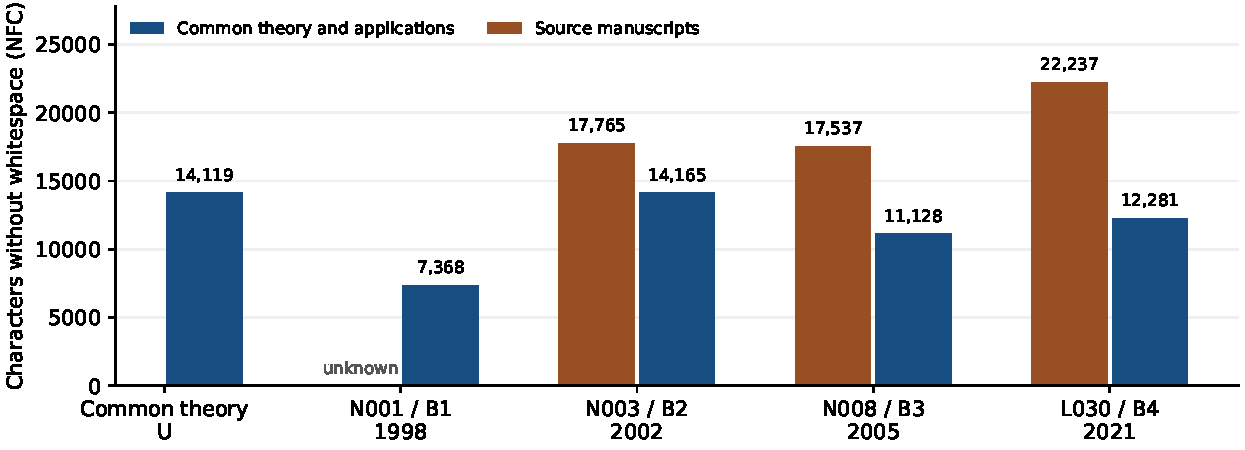
\includegraphics[width=\textwidth]{costs.pdf}
\end{center}
The blank source entry for N001 means unknown; it has no assigned bar
height. The first stage is the common theory, followed by the four
applications. The graph records actual document lengths and makes no
claim of a general pattern of decreasing proof complexity.

\newpage
\section*{What is counted}
Every page is extracted with pypdf 6.13.0, in its original order.
Titles, abstracts, mathematical statements and proofs, references,
addresses, footnotes and unique publication information remain included.
Only the individually recorded running headers and printed page numbers
are removed. Printed hyphens remain; words are not joined across lines.
The five new scientific PDFs comprise 22 pages. The three available
source PDFs comprise 31 pages. Page counts are not used as the headline
length unit. The two-page scope reader supplies audit context and no
mathematical premise; it is identified separately.

The parser represents four pieces of large parentheses on N003 page 8 by
private-use characters. Each is replaced by its visually identified
Unicode hook, preserving four separate pieces. Four open diagram vertices
on L030 page 5 are extracted as the letter i in a circle font; each becomes
a circle character. Every occurrence is bound to its actual font,
page offset and surrounding text. No other substitutions are made.

These rules were checked symmetrically across all eight available source
and replacement PDFs. An independent program re-extracted all 53 pages and
matched all 240 length cells and 48 normalized text hashes. It used independent counting code and rejected changes to the retained text boundary,
page bindings, furniture and glyphs. The same PDF parser remains a shared
dependency of the two counts.

\section*{Units and sensitivity}
The full numerical ledger retains both NFC and NFKC normalization and
three text variants: the complete raw extraction, that extraction after
removing running furniture, and the selected text after glyph correction.
For each it records five units: whitespace-separated tokens, maximal runs
of letters and numbers, characters without whitespace, characters after
collapsing whitespace, and UTF-8 bytes after the same collapse. An underscore
separates such runs. Collapsing whitespace replaces each
internal run by one space and removes leading and trailing whitespace.
The ledger contains ninety exact known conditional fractions, together
with explicit unknown entries for N001 and the complete topic. The
headline coordinate above is fixed in advance of choosing a favorable
factor; all other coordinates remain available in \texttt{results.json}.

\section*{Limits and attribution}
These are lengths of the stated complete documents, not minimum proof
complexities or counts of every visible mark. L030 page 5 has vector graphs
whose edges and layout are not measured. Some graph labels extract despite
being obscured by the drawing. N008's bibliography underline strokes
extract as minus glyphs; they remain counted. N003's original PDF contains
repeated font dictionary keys; the source bytes and parser are fixed, and
its page and font extraction are bound rather than silently repaired.

The foundational Buekenhout--Cara--Dehon classification and the two
separate Whiston results remain substantial retained inputs. Cayley's
formula, the stated symmetric-group automorphism fact, the finite
$p$-group Frattini theorem, Zorn's lemma and elementary linear algebra
also remain explicit. Their expanded proof costs are unknown. Lean
compilation and finite hypothesis counterexamples are verification
infrastructure; they do not supply an omitted mathematical enumeration.
No complete source application is claimed to be formalized in Lean.

This audit preserves the existing source and question credits. The
mathematical admission and corrected source map specify the thirty
clauses being compared; this reader does not expand that scope.
\end{document}
